\documentclass[12pt]{article}

\usepackage{hyperref} %links in ToC
\usepackage{caption} %interesting things with captions
\usepackage[margin=1.5in]{geometry} %mostly set margin of the report
\usepackage{tabulary} %text wrapping in tables
\usepackage{subcaption} %let me put multiple images into a single caption

%images being embeded
\usepackage{graphicx}
\graphicspath{ {images/} }

%code highlighting
\usepackage{minted}
\setminted[c++]{frame=single,linenos=true,autogobble=true,numbersep=4pt,tabsize=4}
\setminted[python]{frame=single,linenos=true,autogobble=true,numbersep=4pt,tabsize=4}
\setminted[bash]{frame=single,linenos=true,autogobble=true,numbersep=4pt,tabsize=4}
\setminted[xml]{frame=single,linenos=true,autogobble=true,numbersep=4pt,tabsize=4}

%fix a quote mark issue
\usepackage [english]{babel}
\usepackage [autostyle, english = american]{csquotes}
\MakeOuterQuote{"}


\begin{document}
\pagenumbering{gobble}
\begin{titlepage}
	\centering
	{\Huge OpenStack\par}
	\vspace{0.25in}
	{\Large Project 2\par}
	\vspace{2in}
	{Alex Harper\par}
	\newpage
\end{titlepage}
\pagenumbering{roman}

\tableofcontents
\newpage

\listoffigures
% \listoftables
\newpage
\setlength{\parindent}{4em} %indent of first line of paragraph
\setlength{\parskip}{1em} %space between paragraphs

\pagenumbering{arabic}

\section{Introduction}

The "cloud" is just a term to say you are using someone elses computers.
To use those computers, there are different pardigms for different people.
The simplest is a VPS where you put the service you want on.
The one large companies do is automated roll out scripts that manage thousands of systems at once.
OpenStack is a group of software that is supposed to help with the latter use case.

When trying to figure out what the software was, I scoured many pages of their website.
So after dashing around the site for a little while, I finally found some information that told me what this thing is. fig\ref{components}

\begin{figure}[ht]
	\centering
	\begin{tabular}{|l|l|}
	\hline
	Nova&VM/Container Managment \\ \hline
	Swift&Abstracted Data Storage \\ \hline
	Cinder&Traditional Data Storage \\ \hline
	Neutron&Networking \\ \hline
	Horizon&Website Control Panel \\ \hline
	Keystone&User Authentication \\ \hline
	Glance&VM/Container Image Host \\ \hline
	Ceilometer&Usage Reporting \\ \hline
	Heat&I Don't Even Know \\ \hline
	\end{tabular}
	\caption{OpenStack Components}
	\label{components}
\end{figure}

Unfortunantly I seem to be completly out of my depth for working with this software.
This paper is short because I had lots of time of not being able to figure out how to get it to work.

\newpage
\section{First Looks}

Before getting into the code, I decided to click every button on the web interface.
The following pictures are what I think different important things are in the side menu.
All the menus are for the current "project" and seem to focus on creating or modifying VMs.

\begin{figure} [ht]
	\centering
	\begin{tabular}{|c|p{0.65\textwidth}|}
		\hline
		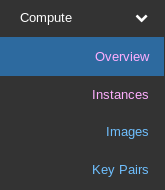
\includegraphics[width=0.2\textwidth]{menu1.png} %overview
		&
		\begin{itemize}
			\vspace{-100pt}
			\item Overview - What resources are being used in the project
			\item Instances - What VMs have been allocated and acces to their configuration
			\item Images - Available boot images for VMs
		\end{itemize}
		\\ \hline
	\end{tabular}

	\begin{tabular}{|c|p{0.65\textwidth}|}
		\hline
		
\includegraphics[width=0.2\textwidth]{menu2.png} %instances
		&
		\begin{itemize}
			\vspace{-100pt}
			\item Volumes - Storage blocks for VMs to use
			\item Backups - List of backups that can be used
		\end{itemize}
		\\ \hline
	\end{tabular}

	\begin{tabular}{|c|p{0.65\textwidth}|}
		\hline
		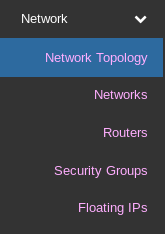
\includegraphics[width=0.2\textwidth]{menu3.png} %images
		&
		\begin{itemize}
			\vspace{-120pt}
			\item Topology - Visual graph of how VMs are connected
			\item Networks - Manage bus-like networks
			\item Routers - Manage connections between networks
			\item Security Groups - Groups with different rules to apply to VMs (firewall)
			\item Floating IPs - Assosiate external IPs to VMs
		\end{itemize}
		\\ \hline
	\end{tabular}
	
	\caption{Project Side Menu}
	\label{side_menu}
\end{figure}

\clearpage
\newpage
So now lets look at the real point of this software, code that can interact with the stack.
Typically using python, you can command the software to various things and dynamicly manage what VMs are running.
This can be useful for different scenarios; increasing capacity during heavy use times, starting a large distributed program, rolling out general VPSs for clients, etc.
From ther perspective of a person with lots of computing hardware, it is nice to have.

The website had a page with example code for getting started with the python code.
It goes through different things for how to have it choose different parameters and setup enviroments for VMs.
Unfortuantly the example code on the site seems to not be entierly in working order.

In order to have the libcloud module communicate with OpenStack, the API version had to be changed to v3.
Apparently my skill at using google is too weak to figure it out on my own.
I had to use the listserv to get someone to help me out.
This was after a few days of trying different things and troublshooting things the way I normally do.
It all started with the example code throwing an exception about "connection refused".

\begin{itemize}
	\item Try various other ports and get various different errors
	\item Check that the user I am using exists
	\item Try making a new user
	\item Reboot the VM and host
	\item Try to find out what I am connecting to
	\begin{itemize}
		\item Service is called Keystone
	\end{itemize}
	\item Check that Keystone is running
	\begin{itemize}
		\item Service shows up as a process
		\item Service does NOT show up as listening on the network
		\item Apache is doing some "ProxyPass" thing to the unix socket
	\end{itemize}
	\item Try different endpoints af the different ports
	\begin{itemize}
		\item Get various different exceptions, most promising ones being 404s
	\end{itemize}
	\item Try to see what OpenStack thinks is running
	\begin{itemize}
		\item try running command "openstack endpoints list"
		\item throws and exception about not being able to find the exception that it wants to throw
	\end{itemize}
	\item Give up on my pride and ask the listserv
	\begin{itemize}
		\item Charles Harper apparently had better google-fu than me this week
		\item Was able to get the most basic example code to work
	\end{itemize}
\end{itemize}

Fantastic, not only can I create a VM from the "dashboard" but also via code.
The instance I had made was using a Ubuntu image.
To test out how well it was working, I decided to SSH into the instance (sub-virtual machine).
The problem with that was trying to get the right IP address.

\begin{itemize}
	\item Instance Private address of 10.0.0.4
	\item Instance Floating IP address of 172.24.4.4
	\item VM address at 192.168.122.237
\end{itemize}

None of the three address above worked for getting into the instance, even from the VM that is running the instance.
Although it is in a security group to allow port 22, I don't thing that it automaticly forwards ports to where it needs to go.
The first place to try to get this to work would be on the VM itself so that I am not trying to coordinate two bridges at the same time.
Unfortunantly I ran out of time to figure it out.
My google skills were not able to find any answers for how to make this work or even if my suspiscions were right.

In general, I consider this whole project a failure.
Not sure what to do about it since I was trying to work but my time was just not effectivly being used.
I am able to create instances though the dashboard and through python code, and it even shows things coming back from the instance.
There just seems to be no way to directly interact with the instance right now.

Below is a picture of the console beig output by the instance, but it does not seem to even take keyboard input.
That means I can't even check that the SSH service is running.
In the appendix is the log from the instance booting, and it shows that the cloudinit service started and pulled some IPs.

\begin{figure}[ht]
	\centering
	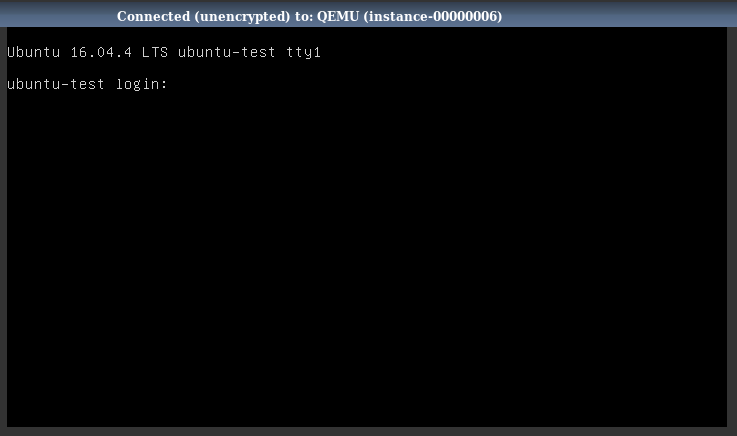
\includegraphics[width=0.8\textwidth]{console.png} %instances
	\caption{Visual Console as shown through the dashboard}
\end{figure}

\appendix
\newpage
\clearpage
\section{Ubuntu Instance Boot Log}
\scriptsize
\begin{verbatim}
[    0.000000] Initializing cgroup subsys cpuset
[    0.000000] Initializing cgroup subsys cpu
[    0.000000] Initializing cgroup subsys cpuacct
[    0.000000] Linux version 4.4.0-116-generic (buildd@lgw01-amd64-021) (gcc version 5.4.0 20160609 (Ubuntu 5.4.0-6ubuntu1~16.04.9) ) #140-Ubuntu SMP Mon Feb 12 21:23:04 UTC 2018 (Ubuntu 4.4.0-116.140-generic 4.4.98)
[    0.000000] Command line: BOOT_IMAGE=/boot/vmlinuz-4.4.0-116-generic root=LABEL=cloudimg-rootfs ro console=tty1 console=ttyS0
[    0.000000] KERNEL supported cpus:
[    0.000000]   Intel GenuineIntel
[    0.000000]   AMD AuthenticAMD
[    0.000000]   Centaur CentaurHauls
[    0.000000] x86/fpu: Legacy x87 FPU detected.
[    0.000000] x86/fpu: Using 'lazy' FPU context switches.
[    0.000000] e820: BIOS-provided physical RAM map:
[    0.000000] BIOS-e820: [mem 0x0000000000000000-0x000000000009fbff] usable
[    0.000000] BIOS-e820: [mem 0x000000000009fc00-0x000000000009ffff] reserved
[    0.000000] BIOS-e820: [mem 0x00000000000f0000-0x00000000000fffff] reserved
[    0.000000] BIOS-e820: [mem 0x0000000000100000-0x000000003ffdbfff] usable
[    0.000000] BIOS-e820: [mem 0x000000003ffdc000-0x000000003fffffff] reserved
[    0.000000] BIOS-e820: [mem 0x00000000fffc0000-0x00000000ffffffff] reserved
[    0.000000] NX (Execute Disable) protection: active
[    0.000000] SMBIOS 2.8 present.
[    0.000000] Kernel/User page tables isolation: disabled
[    0.000000] e820: last_pfn = 0x3ffdc max_arch_pfn = 0x400000000
[    0.000000] x86/PAT: Configuration [0-7]: WB  WC  UC- UC  WB  WC  UC- WT  
[    0.000000] found SMP MP-table at [mem 0x000f6a40-0x000f6a4f] mapped at [ffff8800000f6a40]
[    0.000000] Scanning 1 areas for low memory corruption
[    0.000000] RAMDISK: [mem 0x36ac2000-0x37558fff]
[    0.000000] ACPI: Early table checksum verification disabled
[    0.000000] ACPI: RSDP 0x00000000000F6830 000014 (v00 BOCHS )
[    0.000000] ACPI: RSDT 0x000000003FFE159B 000030 (v01 BOCHS  BXPCRSDT 00000001 BXPC 00000001)
[    0.000000] ACPI: FACP 0x000000003FFE13F7 000074 (v01 BOCHS  BXPCFACP 00000001 BXPC 00000001)
[    0.000000] ACPI: DSDT 0x000000003FFE0040 0013B7 (v01 BOCHS  BXPCDSDT 00000001 BXPC 00000001)
[    0.000000] ACPI: FACS 0x000000003FFE0000 000040
[    0.000000] ACPI: APIC 0x000000003FFE14EB 000078 (v01 BOCHS  BXPCAPIC 00000001 BXPC 00000001)
[    0.000000] ACPI: HPET 0x000000003FFE1563 000038 (v01 BOCHS  BXPCHPET 00000001 BXPC 00000001)
[    0.000000] No NUMA configuration found
[    0.000000] Faking a node at [mem 0x0000000000000000-0x000000003ffdbfff]
[    0.000000] NODE_DATA(0) allocated [mem 0x3ffd7000-0x3ffdbfff]
[    0.000000] Zone ranges:
[    0.000000]   DMA      [mem 0x0000000000001000-0x0000000000ffffff]
[    0.000000]   DMA32    [mem 0x0000000001000000-0x000000003ffdbfff]
[    0.000000]   Normal   empty
[    0.000000]   Device   empty
[    0.000000] Movable zone start for each node
[    0.000000] Early memory node ranges
[    0.000000]   node   0: [mem 0x0000000000001000-0x000000000009efff]
[    0.000000]   node   0: [mem 0x0000000000100000-0x000000003ffdbfff]
[    0.000000] Initmem setup node 0 [mem 0x0000000000001000-0x000000003ffdbfff]
[    0.000000] ACPI: PM-Timer IO Port: 0x608
[    0.000000] ACPI: LAPIC_NMI (acpi_id[0xff] dfl dfl lint[0x1])
[    0.000000] IOAPIC[0]: apic_id 0, version 32, address 0xfec00000, GSI 0-23
[    0.000000] ACPI: INT_SRC_OVR (bus 0 bus_irq 0 global_irq 2 dfl dfl)
[    0.000000] ACPI: INT_SRC_OVR (bus 0 bus_irq 5 global_irq 5 high level)
[    0.000000] ACPI: INT_SRC_OVR (bus 0 bus_irq 9 global_irq 9 high level)
[    0.000000] ACPI: INT_SRC_OVR (bus 0 bus_irq 10 global_irq 10 high level)
[    0.000000] ACPI: INT_SRC_OVR (bus 0 bus_irq 11 global_irq 11 high level)
[    0.000000] Using ACPI (MADT) for SMP configuration information
[    0.000000] ACPI: HPET id: 0x8086a201 base: 0xfed00000
[    0.000000] smpboot: Allowing 1 CPUs, 0 hotplug CPUs
[    0.000000] PM: Registered nosave memory: [mem 0x00000000-0x00000fff]
[    0.000000] PM: Registered nosave memory: [mem 0x0009f000-0x0009ffff]
[    0.000000] PM: Registered nosave memory: [mem 0x000a0000-0x000effff]
[    0.000000] PM: Registered nosave memory: [mem 0x000f0000-0x000fffff]
[    0.000000] e820: [mem 0x40000000-0xfffbffff] available for PCI devices
[    0.000000] Booting paravirtualized kernel on bare hardware
[    0.000000] clocksource: refined-jiffies: mask: 0xffffffff max_cycles: 0xffffffff, max_idle_ns: 7645519600211568 ns
[    0.000000] setup_percpu: NR_CPUS:512 nr_cpumask_bits:512 nr_cpu_ids:1 nr_node_ids:1
[    0.000000] PERCPU: Embedded 34 pages/cpu @ffff88003fc00000 s99544 r8192 d31528 u2097152
[    0.000000] Built 1 zonelists in Node order, mobility grouping on.  Total pages: 257893
[    0.000000] Policy zone: DMA32
[    0.000000] Kernel command line: BOOT_IMAGE=/boot/vmlinuz-4.4.0-116-generic root=LABEL=cloudimg-rootfs ro console=tty1 console=ttyS0
[    0.000000] PID hash table entries: 4096 (order: 3, 32768 bytes)
[    0.000000] Memory: 1001780K/1048040K available (8530K kernel code, 1309K rwdata, 3992K rodata, 1508K init, 1316K bss, 46260K reserved, 0K cma-reserved)
[    0.000000] SLUB: HWalign=64, Order=0-3, MinObjects=0, CPUs=1, Nodes=1
[    0.000000] Hierarchical RCU implementation.
[    0.000000] 	Build-time adjustment of leaf fanout to 64.
[    0.000000] 	RCU restricting CPUs from NR_CPUS=512 to nr_cpu_ids=1.
[    0.000000] RCU: Adjusting geometry for rcu_fanout_leaf=64, nr_cpu_ids=1
[    0.000000] NR_IRQS:33024 nr_irqs:256 16
[    0.000000] Console: colour VGA+ 80x25
[    0.000000] console [tty1] enabled
[    0.000000] console [ttyS0] enabled
[    0.000000] clocksource: hpet: mask: 0xffffffff max_cycles: 0xffffffff, max_idle_ns: 19112604467 ns
[    0.000000] tsc: Fast TSC calibration using PIT
[    0.000000] tsc: Detected 3199.991 MHz processor
[    0.013421] Calibrating delay loop (skipped), value calculated using timer frequency.. 6399.98 BogoMIPS (lpj=12799964)
[    0.016689] pid_max: default: 32768 minimum: 301
[    0.017639] ACPI: Core revision 20150930
[    0.038382] ACPI: 1 ACPI AML tables successfully acquired and loaded
[    0.040752] Security Framework initialized
[    0.041512] Yama: becoming mindful.
[    0.043808] AppArmor: AppArmor initialized
[    0.045969] Dentry cache hash table entries: 131072 (order: 8, 1048576 bytes)
[    0.049228] Inode-cache hash table entries: 65536 (order: 7, 524288 bytes)
[    0.051242] Mount-cache hash table entries: 2048 (order: 2, 16384 bytes)
[    0.052082] Mountpoint-cache hash table entries: 2048 (order: 2, 16384 bytes)
[    0.062063] Initializing cgroup subsys io
[    0.063295] Initializing cgroup subsys memory
[    0.064567] Initializing cgroup subsys devices
[    0.065545] Initializing cgroup subsys freezer
[    0.066517] Initializing cgroup subsys net_cls
[    0.067444] Initializing cgroup subsys perf_event
[    0.068099] Initializing cgroup subsys net_prio
[    0.068973] Initializing cgroup subsys hugetlb
[    0.069814] Initializing cgroup subsys pids
[    0.072418] FEATURE SPEC_CTRL Not Present
[    0.073124] FEATURE IBPB Not Present
[    0.073961] mce: CPU supports 10 MCE banks
[    0.075737] Last level iTLB entries: 4KB 0, 2MB 0, 4MB 0
[    0.076043] Last level dTLB entries: 4KB 0, 2MB 0, 4MB 0, 1GB 0
[    0.077227] Spectre V2 mitigation: Mitigation: Full AMD retpoline
[    0.078400] Spectre V2 mitigation: Speculation control IBPB not-supported IBRS not-supported
[    0.413937] Freeing SMP alternatives memory: 32K
[    0.425224] ftrace: allocating 32186 entries in 126 pages
[    0.489847] smpboot: APIC(0) Converting physical 0 to logical package 0
[    0.491459] smpboot: Max logical packages: 1
[    0.495887] ..TIMER: vector=0x30 apic1=0 pin1=2 apic2=-1 pin2=-1
[    0.540000] smpboot: CPU0: AMD QEMU Virtual CPU version 2.5+ (family: 0x6, model: 0x6, stepping: 0x3)
[    0.540000] Performance Events: Broken PMU hardware detected, using software events only.
[    0.540081] Failed to access perfctr msr (MSR c0010007 is 0)
[    0.551976] x86: Booted up 1 node, 1 CPUs
[    0.552115] smpboot: Total of 1 processors activated (6399.98 BogoMIPS)
[    0.558382] NMI watchdog: disabled (cpu0): hardware events not enabled
[    0.559767] NMI watchdog: Shutting down hard lockup detector on all cpus
[    0.569984] devtmpfs: initialized
[    0.586029] evm: security.selinux
[    0.586782] evm: security.SMACK64
[    0.587407] evm: security.SMACK64EXEC
[    0.588040] evm: security.SMACK64TRANSMUTE
[    0.588724] evm: security.SMACK64MMAP
[    0.589339] evm: security.ima
[    0.589902] evm: security.capability
[    0.593482] clocksource: jiffies: mask: 0xffffffff max_cycles: 0xffffffff, max_idle_ns: 7645041785100000 ns
[    0.595521] futex hash table entries: 256 (order: 2, 16384 bytes)
[    0.598393] pinctrl core: initialized pinctrl subsystem
[    0.605812] RTC time: 19:29:34, date: 03/19/18
[    0.611445] NET: Registered protocol family 16
[    0.616630] cpuidle: using governor ladder
[    0.617546] cpuidle: using governor menu
[    0.618482] PCCT header not found.
[    0.620307] ACPI: bus type PCI registered
[    0.621089] acpiphp: ACPI Hot Plug PCI Controller Driver version: 0.5
[    0.624110] PCI: Using configuration type 1 for base access
[    0.645341] ACPI: Added _OSI(Module Device)
[    0.646283] ACPI: Added _OSI(Processor Device)
[    0.647146] ACPI: Added _OSI(3.0 _SCP Extensions)
[    0.648036] ACPI: Added _OSI(Processor Aggregator Device)
[    0.665535] ACPI: Interpreter enabled
[    0.667019] ACPI: (supports S0 S3 S4 S5)
[    0.667817] ACPI: Using IOAPIC for interrupt routing
[    0.668407] PCI: Using host bridge windows from ACPI; if necessary, use "pci=nocrs" and report a bug
[    0.702940] ACPI: PCI Root Bridge [PCI0] (domain 0000 [bus 00-ff])
[    0.704390] acpi PNP0A03:00: _OSC: OS supports [ASPM ClockPM Segments MSI]
[    0.705776] acpi PNP0A03:00: _OSC failed (AE_NOT_FOUND); disabling ASPM
[    0.707479] acpi PNP0A03:00: fail to add MMCONFIG information, can't access extended PCI configuration space under this bridge.
[    0.715093] acpiphp: Slot [3] registered
[    0.716293] acpiphp: Slot [4] registered
[    0.717296] acpiphp: Slot [5] registered
[    0.719116] acpiphp: Slot [6] registered
[    0.720217] acpiphp: Slot [7] registered
[    0.721083] acpiphp: Slot [8] registered
[    0.721872] acpiphp: Slot [9] registered
[    0.722743] acpiphp: Slot [10] registered
[    0.723644] acpiphp: Slot [11] registered
[    0.724169] acpiphp: Slot [12] registered
[    0.725093] acpiphp: Slot [13] registered
[    0.725949] acpiphp: Slot [14] registered
[    0.726861] acpiphp: Slot [15] registered
[    0.728144] acpiphp: Slot [16] registered
[    0.728915] acpiphp: Slot [17] registered
[    0.729704] acpiphp: Slot [18] registered
[    0.730563] acpiphp: Slot [19] registered
[    0.731416] acpiphp: Slot [20] registered
[    0.732139] acpiphp: Slot [21] registered
[    0.732935] acpiphp: Slot [22] registered
[    0.733799] acpiphp: Slot [23] registered
[    0.734660] acpiphp: Slot [24] registered
[    0.736139] acpiphp: Slot [25] registered
[    0.736968] acpiphp: Slot [26] registered
[    0.737774] acpiphp: Slot [27] registered
[    0.738707] acpiphp: Slot [28] registered
[    0.739594] acpiphp: Slot [29] registered
[    0.740150] acpiphp: Slot [30] registered
[    0.740981] acpiphp: Slot [31] registered
[    0.742077] PCI host bridge to bus 0000:00
[    0.743008] pci_bus 0000:00: root bus resource [io  0x0000-0x0cf7 window]
[    0.744066] pci_bus 0000:00: root bus resource [io  0x0d00-0xffff window]
[    0.745172] pci_bus 0000:00: root bus resource [mem 0x000a0000-0x000bffff window]
[    0.746656] pci_bus 0000:00: root bus resource [mem 0x40000000-0xfebfffff window]
[    0.748129] pci_bus 0000:00: root bus resource [bus 00-ff]
[    0.759014] pci 0000:00:01.1: legacy IDE quirk: reg 0x10: [io  0x01f0-0x01f7]
[    0.760079] pci 0000:00:01.1: legacy IDE quirk: reg 0x14: [io  0x03f6]
[    0.761234] pci 0000:00:01.1: legacy IDE quirk: reg 0x18: [io  0x0170-0x0177]
[    0.762522] pci 0000:00:01.1: legacy IDE quirk: reg 0x1c: [io  0x0376]
[    0.772593] pci 0000:00:01.3: quirk: [io  0x0600-0x063f] claimed by PIIX4 ACPI
[    0.773881] pci 0000:00:01.3: quirk: [io  0x0700-0x070f] claimed by PIIX4 SMB
[    0.826887] ACPI: PCI Interrupt Link [LNKA] (IRQs 5 *10 11)
[    0.828928] ACPI: PCI Interrupt Link [LNKB] (IRQs 5 *10 11)
[    0.830514] ACPI: PCI Interrupt Link [LNKC] (IRQs 5 10 *11)
[    0.832675] ACPI: PCI Interrupt Link [LNKD] (IRQs 5 10 *11)
[    0.833975] ACPI: PCI Interrupt Link [LNKS] (IRQs *9)
[    0.836924] ACPI: Enabled 2 GPEs in block 00 to 0F
[    0.841329] vgaarb: setting as boot device: PCI:0000:00:02.0
[    0.842617] vgaarb: device added: PCI:0000:00:02.0,decodes=io+mem,owns=io+mem,locks=none
[    0.844064] vgaarb: loaded
[    0.844608] vgaarb: bridge control possible 0000:00:02.0
[    0.849028] SCSI subsystem initialized
[    0.850913] ACPI: bus type USB registered
[    0.852203] usbcore: registered new interface driver usbfs
[    0.853334] usbcore: registered new interface driver hub
[    0.854522] usbcore: registered new device driver usb
[    0.857883] PCI: Using ACPI for IRQ routing
[    0.864688] NetLabel: Initializing
[    0.865320] NetLabel:  domain hash size = 128
[    0.866132] NetLabel:  protocols = UNLABELED CIPSOv4
[    0.868047] NetLabel:  unlabeled traffic allowed by default
[    0.870028] HPET: 3 timers in total, 0 timers will be used for per-cpu timer
[    0.871494] hpet0: at MMIO 0xfed00000, IRQs 2, 8, 0
[    0.872379] hpet0: 3 comparators, 64-bit 100.000000 MHz counter
[    0.878180] amd_nb: Cannot enumerate AMD northbridges
[    0.880522] clocksource: Switched to clocksource hpet
[    0.967715] AppArmor: AppArmor Filesystem Enabled
[    0.970257] pnp: PnP ACPI init
[    0.975854] pnp: PnP ACPI: found 5 devices
[    1.002899] clocksource: acpi_pm: mask: 0xffffff max_cycles: 0xffffff, max_idle_ns: 2085701024 ns
[    1.005895] NET: Registered protocol family 2
[    1.011503] TCP established hash table entries: 8192 (order: 4, 65536 bytes)
[    1.013185] TCP bind hash table entries: 8192 (order: 5, 131072 bytes)
[    1.014549] TCP: Hash tables configured (established 8192 bind 8192)
[    1.016514] UDP hash table entries: 512 (order: 2, 16384 bytes)
[    1.017684] UDP-Lite hash table entries: 512 (order: 2, 16384 bytes)
[    1.020247] NET: Registered protocol family 1
[    1.021349] pci 0000:00:00.0: Limiting direct PCI/PCI transfers
[    1.022419] pci 0000:00:01.0: PIIX3: Enabling Passive Release
[    1.023525] pci 0000:00:01.0: Activating ISA DMA hang workarounds
[    1.192601] ACPI: PCI Interrupt Link [LNKD] enabled at IRQ 11
[    1.375511] Unpacking initramfs...
[   13.197689] Freeing initrd memory: 10844K
[   13.200934] Scanning for low memory corruption every 60 seconds
[   13.205967] audit: initializing netlink subsys (disabled)
[   13.207522] audit: type=2000 audit(1521487787.204:1): initialized
[   13.211584] Initialise system trusted keyring
[   13.214708] HugeTLB registered 2 MB page size, pre-allocated 0 pages
[   13.229621] zbud: loaded
[   13.232662] VFS: Disk quotas dquot_6.6.0
[   13.233766] VFS: Dquot-cache hash table entries: 512 (order 0, 4096 bytes)
[   13.240235] squashfs: version 4.0 (2009/01/31) Phillip Lougher
[   13.244731] fuse init (API version 7.23)
[   13.247504] Key type big_key registered
[   13.248666] Allocating IMA MOK and blacklist keyrings.
[   13.256462] Key type asymmetric registered
[   13.257308] Asymmetric key parser 'x509' registered
[   13.258744] Block layer SCSI generic (bsg) driver version 0.4 loaded (major 249)
[   13.260891] io scheduler noop registered
[   13.261742] io scheduler deadline registered (default)
[   13.263217] io scheduler cfq registered
[   13.266393] pci_hotplug: PCI Hot Plug PCI Core version: 0.5
[   13.267651] pciehp: PCI Express Hot Plug Controller Driver version: 0.4
[   13.272069] input: Power Button as /devices/LNXSYSTM:00/LNXPWRBN:00/input/input0
[   13.273930] ACPI: Power Button [PWRF]
[   13.277294] GHES: HEST is not enabled!
[   13.442702] ACPI: PCI Interrupt Link [LNKC] enabled at IRQ 10
[   13.760487] ACPI: PCI Interrupt Link [LNKA] enabled at IRQ 10
[   13.766295] Serial: 8250/16550 driver, 32 ports, IRQ sharing enabled
[   13.792385] 00:04: ttyS0 at I/O 0x3f8 (irq = 4, base_baud = 115200) is a 16550A
[   13.808839] Linux agpgart interface v0.103
[   13.829906] loop: module loaded
[   13.851609]  vda: vda1
[   13.863394] scsi host0: ata_piix
[   13.865418] scsi host1: ata_piix
[   13.866571] ata1: PATA max MWDMA2 cmd 0x1f0 ctl 0x3f6 bmdma 0xc0a0 irq 14
[   13.867944] ata2: PATA max MWDMA2 cmd 0x170 ctl 0x376 bmdma 0xc0a8 irq 15
[   13.873192] libphy: Fixed MDIO Bus: probed
[   13.874050] tun: Universal TUN/TAP device driver, 1.6
[   13.874980] tun: (C) 1999-2004 Max Krasnyansky <maxk@qualcomm.com>
[   13.883925] PPP generic driver version 2.4.2
[   13.885781] ehci_hcd: USB 2.0 'Enhanced' Host Controller (EHCI) Driver
[   13.887323] ehci-pci: EHCI PCI platform driver
[   13.888606] ehci-platform: EHCI generic platform driver
[   13.889751] ohci_hcd: USB 1.1 'Open' Host Controller (OHCI) Driver
[   13.891077] ohci-pci: OHCI PCI platform driver
[   13.892251] ohci-platform: OHCI generic platform driver
[   13.893428] uhci_hcd: USB Universal Host Controller Interface driver
[   14.055093] uhci_hcd 0000:00:01.2: UHCI Host Controller
[   14.056777] uhci_hcd 0000:00:01.2: new USB bus registered, assigned bus number 1
[   14.058719] uhci_hcd 0000:00:01.2: detected 2 ports
[   14.060233] uhci_hcd 0000:00:01.2: irq 11, io base 0x0000c040
[   14.065052] usb usb1: New USB device found, idVendor=1d6b, idProduct=0001
[   14.066578] usb usb1: New USB device strings: Mfr=3, Product=2, SerialNumber=1
[   14.068283] usb usb1: Product: UHCI Host Controller
[   14.069396] usb usb1: Manufacturer: Linux 4.4.0-116-generic uhci_hcd
[   14.070731] usb usb1: SerialNumber: 0000:00:01.2
[   14.074701] hub 1-0:1.0: USB hub found
[   14.076248] hub 1-0:1.0: 2 ports detected
[   14.082746] i8042: PNP: PS/2 Controller [PNP0303:KBD,PNP0f13:MOU] at 0x60,0x64 irq 1,12
[   14.087512] serio: i8042 KBD port at 0x60,0x64 irq 1
[   14.088880] serio: i8042 AUX port at 0x60,0x64 irq 12
[   14.092320] mousedev: PS/2 mouse device common for all mice
[   14.096322] input: AT Translated Set 2 keyboard as /devices/platform/i8042/serio0/input/input1
[   14.099331] rtc_cmos 00:00: RTC can wake from S4
[   14.103038] rtc_cmos 00:00: rtc core: registered rtc_cmos as rtc0
[   14.105074] rtc_cmos 00:00: alarms up to one day, y3k, 114 bytes nvram, hpet irqs
[   14.106863] i2c /dev entries driver
[   14.108414] device-mapper: uevent: version 1.0.3
[   14.110488] device-mapper: ioctl: 4.34.0-ioctl (2015-10-28) initialised: dm-devel@redhat.com
[   14.113736] ledtrig-cpu: registered to indicate activity on CPUs
[   14.118311] NET: Registered protocol family 10
[   14.125521] NET: Registered protocol family 17
[   14.133742] Key type dns_resolver registered
[   14.139567] microcode: AMD CPU family 0x6 not supported
[   14.146179] registered taskstats version 1
[   14.147314] Loading compiled-in X.509 certificates
[   14.162843] Loaded X.509 cert 'Build time autogenerated kernel key: aa84f01984fbd529c105810b59e379d349698248'
[   14.166043] zswap: loaded using pool lzo/zbud
[   14.203698] tsc: Refined TSC clocksource calibration: 3199.991 MHz
[   14.205324] clocksource: tsc: mask: 0xffffffffffffffff max_cycles: 0x2e2041630d7, max_idle_ns: 440795278720 ns
[   14.307752] Key type trusted registered
[   14.437294] Key type encrypted registered
[   14.438291] AppArmor: AppArmor sha1 policy hashing enabled
[   14.439623] ima: No TPM chip found, activating TPM-bypass!
[   14.442517] evm: HMAC attrs: 0x1
[   14.445538]   Magic number: 10:351:496
[   14.447036] rtc_cmos 00:00: setting system clock to 2018-03-19 19:29:48 UTC (1521487788)
[   14.450910] BIOS EDD facility v0.16 2004-Jun-25, 0 devices found
[   14.452413] EDD information not available.
[   14.494490] Freeing unused kernel memory: 1508K
[   14.495585] Write protecting the kernel read-only data: 14336k
[   14.499538] Freeing unused kernel memory: 1700K
[   14.502282] Freeing unused kernel memory: 104K
Loading, please wait...
starting version 229
[   14.929889] random: systemd-udevd: uninitialized urandom read (16 bytes read, 5 bits of entropy available)
[   14.951005] random: systemd-udevd: uninitialized urandom read (16 bytes read, 5 bits of entropy available)
[   14.957404] random: systemd-udevd: uninitialized urandom read (16 bytes read, 5 bits of entropy available)
[   14.959824] random: systemd-udevd: uninitialized urandom read (16 bytes read, 5 bits of entropy available)
[   14.978838] random: udevadm: uninitialized urandom read (16 bytes read, 5 bits of entropy available)
[   14.990117] random: udevadm: uninitialized urandom read (16 bytes read, 5 bits of entropy available)
[   15.116575] random: systemd-udevd: uninitialized urandom read (16 bytes read, 5 bits of entropy available)
[   15.119464] random: systemd-udevd: uninitialized urandom read (16 bytes read, 5 bits of entropy available)
[   15.124676] random: systemd-udevd: uninitialized urandom read (16 bytes read, 5 bits of entropy available)
[   15.149854] random: systemd-udevd: uninitialized urandom read (16 bytes read, 5 bits of entropy available)
[   15.216888] clocksource: Switched to clocksource tsc
[   16.477861] FDC 0 is a S82078B
[   16.560934] virtio_net virtio0 ens3: renamed from eth0
[   17.658407] input: ImExPS/2 Generic Explorer Mouse as /devices/platform/i8042/serio1/input/input3
Begin: Loading essential drivers ... [   20.159831] md: linear personality registered for level -1
[   20.212490] md: multipath personality registered for level -4
[   20.272522] md: raid0 personality registered for level 0
[   20.334120] md: raid1 personality registered for level 1
[   20.472232] raid6: sse2x1   gen()   538 MB/s
[   20.540520] raid6: sse2x1   xor()   286 MB/s
[   20.608130] raid6: sse2x2   gen()   612 MB/s
[   20.676160] raid6: sse2x2   xor()   337 MB/s
[   20.744152] raid6: sse2x4   gen()   621 MB/s
[   20.812129] raid6: sse2x4   xor()   342 MB/s
[   20.813045] raid6: using algorithm sse2x4 gen() 621 MB/s
[   20.814013] raid6: .... xor() 342 MB/s, rmw enabled
[   20.815147] raid6: using intx1 recovery algorithm
[   20.836929] xor: measuring software checksum speed
[   20.876173]    prefetch64-sse:  1297.000 MB/sec
[   20.916128]    generic_sse:  1293.000 MB/sec
[   20.917066] xor: using function: prefetch64-sse (1297.000 MB/sec)
[   20.933083] async_tx: api initialized (async)
[   21.024923] md: raid6 personality registered for level 6
[   21.026193] md: raid5 personality registered for level 5
[   21.027268] md: raid4 personality registered for level 4
[   21.168553] md: raid10 personality registered for level 10
done.
Begin: Running /scripts/init-premount ... done.
Begin: Mounting root file system ... Begin: Running /scripts/local-top ... done.
Begin: Running /scripts/local-premount ... [   21.603021] Btrfs loaded
Scanning for Btrfs filesystems
done.
Warning: fsck not present, so skipping root file system
[   22.089445] EXT4-fs (vda1): mounted filesystem with ordered data mode. Opts: (null)
done.
Begin: Running /scripts/local-bottom ... done.
Begin: Running /scripts/init-bottom ... done.
[   23.320745] systemd[1]: systemd 229 running in system mode. (+PAM +AUDIT +SELINUX +IMA +APPARMOR +SMACK +SYSVINIT +UTMP +LIBCRYPTSETUP +GCRYPT +GNUTLS +ACL +XZ -LZ4 +SECCOMP +BLKID +ELFUTILS +KMOD -IDN)
[   23.326406] systemd[1]: Detected virtualization vm-other.
[   23.327763] systemd[1]: Detected architecture x86-64.

Welcome to [1mUbuntu 16.04.4 LTS[0m!

[   23.340222] systemd[1]: Set hostname to <ubuntu-test>.
[   25.223730] systemd[1]: Started Forward Password Requests to Wall Directory Watch.
[[0;32m  OK  [0m] Started Forward Password Requests to Wall Directory Watch.
[   25.242781] systemd[1]: Reached target User and Group Name Lookups.
[[0;32m  OK  [0m] Reached target User and Group Name Lookups.
[   25.247445] systemd[1]: Started Trigger resolvconf update for networkd DNS.
[[0;32m  OK  [0m] Started Trigger resolvconf update for networkd DNS.
[   25.254461] systemd[1]: Listening on Journal Socket.
[[0;32m  OK  [0m] Listening on Journal Socket.
[   25.258241] systemd[1]: Reached target Encrypted Volumes.
[[0;32m  OK  [0m] Reached target Encrypted Volumes.
[   25.265983] systemd[1]: Listening on Device-mapper event daemon FIFOs.
[[0;32m  OK  [0m] Listening on Device-mapper event daemon FIFOs.
[   25.270641] systemd[1]: Listening on LVM2 poll daemon socket.
[[0;32m  OK  [0m] Listening on LVM2 poll daemon socket.
[   25.276841] systemd[1]: Listening on udev Kernel Socket.
[[0;32m  OK  [0m] Listening on udev Kernel Socket.
[   25.290298] systemd[1]: Set up automount Arbitrary Executable File Formats File System Automount Point.
[[0;32m  OK  [0m] Set up automount Arbitrary Executab...ats File System Automount Point.
[   25.295661] systemd[1]: Reached target Swap.
[[0;32m  OK  [0m] Reached target Swap.
[   25.299276] systemd[1]: Listening on /dev/initctl Compatibility Named Pipe.
[[0;32m  OK  [0m] Listening on /dev/initctl Compatibility Named Pipe.
[   25.304525] systemd[1]: Listening on Syslog Socket.
[[0;32m  OK  [0m] Listening on Syslog Socket.
[   25.307805] systemd[1]: Listening on LVM2 metadata daemon socket.
[[0;32m  OK  [0m] Listening on LVM2 metadata daemon socket.
[   25.313389] systemd[1]: Listening on udev Control Socket.
[[0;32m  OK  [0m] Listening on udev Control Socket.
[   25.317211] systemd[1]: Listening on Journal Socket (/dev/log).
[[0;32m  OK  [0m] Listening on Journal Socket (/dev/log).
[   25.334027] systemd[1]: Created slice User and Session Slice.
[[0;32m  OK  [0m] Created slice User and Session Slice.
[   25.342222] systemd[1]: Created slice System Slice.
[[0;32m  OK  [0m] Created slice System Slice.
[   25.385343] systemd[1]: Starting Set console keymap...
         Starting Set console keymap...
[   25.454296] systemd[1]: Starting Load Kernel Modules...
         Starting Load Kernel Modules...
[   25.535728] systemd[1]: Mounting Debug File System...
         Mounting Debug File System...
[   25.725495] systemd[1]: Starting Uncomplicated firewall...
         Starting Uncomplicated firewall...
[   25.887142] systemd[1]: Starting Nameserver information manager...
         Starting Nameserver information manager...
[   26.013968] systemd[1]: Starting Monitoring of LVM2 mirrors, snapshots etc. using dmeventd or progress polling...
         Starting Monitoring of LVM2 mirrors... dmeventd or progress polling...
[   26.186123] systemd[1]: Starting Create list of required static device nodes for the current kernel...
         Starting Create list of required st... nodes for the current kernel...
[   26.244715] systemd[1]: Reached target Slices.
[[0;32m  OK  [0m] Reached target Slices.
[   26.386448] systemd[1]: Starting Remount Root and Kernel File Systems...
         Starting Remount Root and Kernel File Systems...
[   26.513656] systemd[1]: Mounting Huge Pages File System...
         Mounting Huge Pages File System...
[   26.593884] systemd[1]: Created slice system-serial\x2dgetty.slice.
[[0;32m  OK  [0m] Created slice system-serial\x2dgetty.slice.
[   26.630437] systemd[1]: Listening on Journal Audit Socket.
[[0;32m  OK  [0m] Listening on Journal Audit Socket.
[   26.703871] systemd[1]: Starting Journal Service...
         Starting Journal Service...
[   26.791866] systemd[1]: Mounting POSIX Message Queue File System...
         Mounting POSIX Message Queue File System...
[   27.698502] systemd[1]: Started Uncomplicated firewall.
[[0;32m  OK  [0m] Started Uncomplicated firewall.
[   27.770221] systemd[1]: Started Create list of required static device nodes for the current kernel.
[[0;32m  OK  [0m] Started Create list of required sta...ce nodes for the current kernel.
[   27.999260] systemd[1]: Mounted Debug File System.
[[0;32m  OK  [0m] Mounted Debug File System.
[   28.343042] systemd[1]: Mounted Huge Pages File System.
[[0;32m  OK  [0m] Mounted Huge Pages File System.
[   28.386810] systemd[1]: Mounted POSIX Message Queue File System.
[[0;32m  OK  [0m] Mounted POSIX Message Queue File System.
[   28.670122] Loading iSCSI transport class v2.0-870.
[   28.711277] systemd[1]: Started Nameserver information manager.
[[0;32m  OK  [0m] Started Nameserver information manager.
[   29.279720] iscsi: registered transport (tcp)
[   29.433728] EXT4-fs (vda1): re-mounted. Opts: (null)
[   29.480964] systemd[1]: Started Remount Root and Kernel File Systems.
[[0;32m  OK  [0m] Started Remount Root and Kernel File Systems.
[   30.233993] iscsi: registered transport (iser)
[   30.300811] systemd[1]: Started Load Kernel Modules.
[[0;32m  OK  [0m] Started Load Kernel Modules.
[   30.403096] systemd[1]: Starting Apply Kernel Variables...
         Starting Apply Kernel Variables...
[   30.447355] systemd[1]: Mounting FUSE Control File System...
         Mounting FUSE Control File System...
[   30.558211] systemd[1]: Started LVM2 metadata daemon.
[[0;32m  OK  [0m] Started LVM2 metadata daemon.
[   30.724708] systemd[1]: Starting udev Coldplug all Devices...
         Starting udev Coldplug all Devices...
[   30.838744] systemd[1]: Starting Initial cloud-init job (pre-networking)...
         Starting Initial cloud-init job (pre-networking)...
[   30.982493] systemd[1]: Starting Load/Save Random Seed...
         Starting Load/Save Random Seed...
[   31.121670] systemd[1]: Starting Create Static Device Nodes in /dev...
         Starting Create Static Device Nodes in /dev...
[   31.959035] systemd[1]: Mounted FUSE Control File System.
[[0;32m  OK  [0m] Mounted FUSE Control File System.
[[0;32m  OK  [0m] Started Load/Save Random Seed.
[[0;32m  OK  [0m] Started Apply Kernel Variables.
[[0;32m  OK  [0m] Started Journal Service.
         Starting Flush Journal to Persistent Storage...
[[0;32m  OK  [0m] Started Create Static Device Nodes in /dev.
         Starting udev Kernel Device Manager...
[[0;32m  OK  [0m] Started Flush Journal to Persistent Storage.
[[0;32m  OK  [0m] Started Monitoring of LVM2 mirrors,...ng dmeventd or progress polling.
[[0;32m  OK  [0m] Started udev Kernel Device Manager.
[[0;32m  OK  [0m] Started Set console keymap.
[[0;32m  OK  [0m] Reached target Local File Systems (Pre).
[[0;32m  OK  [0m] Reached target Local File Systems.
         Starting Set console font and keymap...
         Starting Tell Plymouth To Write Out Runtime Data...
         Starting Create Volatile Files and Directories...
         Starting LSB: AppArmor initialization...
[[0;32m  OK  [0m] Started Tell Plymouth To Write Out Runtime Data.
[[0;32m  OK  [0m] Started Create Volatile Files and Directories.
         Starting Network Time Synchronization...
         Starting Update UTMP about System Boot/Shutdown...
[[0;32m  OK  [0m] Started Update UTMP about System Boot/Shutdown.
[[0;32m  OK  [0m] Started udev Coldplug all Devices.
[[0;32m  OK  [0m] Started Dispatch Password Requests to Console Directory Watch.
[[0;32m  OK  [0m] Started Network Time Synchronization.
[[0;32m  OK  [0m] Reached target System Time Synchronized.
[[0;32m  OK  [0m] Started LSB: AppArmor initialization.
[[0;32m  OK  [0m] Started Set console font and keymap.
[[0;32m  OK  [0m] Created slice system-getty.slice.
[[0;32m  OK  [0m] Found device /dev/ttyS0.
[[0;32m  OK  [0m] Listening on Load/Save RF Kill Switch Status /dev/rfkill Watch.
[   61.583841] cloud-init[407]: Cloud-init v. 17.2 running 'init-local' at Mon, 19 Mar 2018 19:30:29 +0000. Up 55.30 seconds.
[[0;32m  OK  [0m] Started Initial cloud-init job (pre-networking).
[[0;32m  OK  [0m] Reached target Network (Pre).
         Starting Raise network interfaces...
[[0;32m  OK  [0m] Started ifup for ens3.
[[0;32m  OK  [0m] Found device Virtio network device.
[[0;31m*[0;1;31m*[0m[0;31m*   [0m] A start job is running for Raise network interfaces (43s / 5min 40s)[K[ [0;31m*[0;1;31m*[0m[0;31m*  [0m] A start job is running for Raise network interfaces (44s / 5min 40s)[K[  [0;31m*[0;1;31m*[0m[0;31m* [0m] A start job is running for Raise network interfaces (44s / 5min 40s)[K[   [0;31m*[0;1;31m*[0m[0;31m*[0m] A start job is running for Raise network interfaces (45s / 5min 40s)[K[    [0;31m*[0;1;31m*[0m] A start job is running for Raise network interfaces (45s / 5min 40s)[K[[0;32m  OK  [0m] Started Raise network interfaces.
[[0;32m  OK  [0m] Reached target Network.
         Starting Initial cloud-init job (metadata service crawler)...
[   81.435876] cloud-init[921]: Cloud-init v. 17.2 running 'init' at Mon, 19 Mar 2018 19:30:50 +0000. Up 76.30 seconds.
[   81.498667] cloud-init[921]: ci-info: +++++++++++++++++++++++++++++++++++++++++++++Net device info++++++++++++++++++++++++++++++++++++++++++++++
[   81.511610] cloud-init[921]: ci-info: +--------+------+-----------------------------------------+-----------------+--------+-------------------+
[   81.522512] cloud-init[921]: ci-info: | Device |  Up  |                 Address                 |       Mask      | Scope  |     Hw-Address    |
[   81.534958] cloud-init[921]: ci-info: +--------+------+-----------------------------------------+-----------------+--------+-------------------+
[   81.546541] cloud-init[921]: ci-info: |  ens3  | True |                 10.0.0.4                | 255.255.255.192 |   .    | fa:16:3e:6f:60:3f |
[   81.559729] cloud-init[921]: ci-info: |  ens3  | True | fdd6:996a:974c:0:f816:3eff:fe6f:603f/64 |        .        | global | fa:16:3e:6f:60:3f |
[   81.574764] cloud-init[921]: ci-info: |   lo   | True |                127.0.0.1                |    255.0.0.0    |   .    |         .         |
[   81.590280] cloud-init[921]: ci-info: |   lo   | True |                 ::1/128                 |        .        |  host  |         .         |
[   81.602356] cloud-init[921]: ci-info: +--------+------+-----------------------------------------+-----------------+--------+-------------------+
[   81.611331] cloud-init[921]: ci-info: ++++++++++++++++++++++++++++++Route IPv4 info+++++++++++++++++++++++++++++++
[   81.626243] cloud-init[921]: ci-info: +-------+-----------------+----------+-----------------+-----------+-------+
[   81.634804] cloud-init[921]: ci-info: | Route |   Destination   | Gateway  |     Genmask     | Interface | Flags |
[   81.646708] cloud-init[921]: ci-info: +-------+-----------------+----------+-----------------+-----------+-------+
[   81.658287] cloud-init[921]: ci-info: |   0   |     0.0.0.0     | 10.0.0.1 |     0.0.0.0     |    ens3   |   UG  |
[   81.670917] cloud-init[921]: ci-info: |   1   |     10.0.0.0    | 0.0.0.0  | 255.255.255.192 |    ens3   |   U   |
[   81.685616] cloud-init[921]: ci-info: |   2   | 169.254.169.254 | 10.0.0.1 | 255.255.255.255 |    ens3   |  UGH  |
[   81.695167] cloud-init[921]: ci-info: +-------+-----------------+----------+-----------------+-----------+-------+
[[0;32m  OK  [0m] Started Initial cloud-init job (metadata service crawler).
[[0;32m  OK  [0m] Reached target Network is Online.
         Starting iSCSI initiator daemon (iscsid)...
[[0;32m  OK  [0m] Reached target Cloud-config availability.
[[0;32m  OK  [0m] Reached target System Initialization.
         Starting LXD - unix socket.
[[0;32m  OK  [0m] Started Daily apt download activities.
[[0;32m  OK  [0m] Started Daily apt upgrade and clean activities.
[[0;32m  OK  [0m] Listening on UUID daemon activation socket.
[[0;32m  OK  [0m] Started Timer to automatically refresh installed snaps.
[[0;32m  OK  [0m] Started ACPI Events Check.
[[0;32m  OK  [0m] Reached target Paths.
[[0;32m  OK  [0m] Listening on D-Bus System Message Bus Socket.
[[0;32m  OK  [0m] Listening on ACPID Listen Socket.
[[0;32m  OK  [0m] Started Daily Cleanup of Temporary Directories.
[[0;32m  OK  [0m] Reached target Timers.
         Starting Socket activation for snappy daemon.
[[0;32m  OK  [0m] Listening on LXD - unix socket.
[[0;32m  OK  [0m] Listening on Socket activation for snappy daemon.
[[0;32m  OK  [0m] Reached target Sockets.
[[0;32m  OK  [0m] Reached target Basic System.
         Starting /etc/rc.local Compatibility...
         Starting LSB: MD monitoring daemon...
[[0;32m  OK  [0m] Started Regular background program processing daemon.
         Starting Accounts Service...
         Starting Apply the settings specified in cloud-config...
[[0;32m  OK  [0m] Started D-Bus System Message Bus.
         Starting System Logging Service...
[[0;32m  OK  [0m] Started FUSE filesystem for LXC.
[[0;32m  OK  [0m] Started ACPI event daemon.
[[0;32m  OK  [0m] Started Deferred execution scheduler.
[[0;32m  OK  [0m] Started Unattended Upgrades Shutdown.
         Starting Login Service...
         Starting Pollinate to seed the pseudo random number generator...
         Starting Snappy daemon...
         Starting LSB: Record successful boot for GRUB...
         Starting LXD - container startup/shutdown...
[[0;32m  OK  [0m] Started iSCSI initiator daemon (iscsid).
[[0;32m  OK  [0m] Started /etc/rc.local Compatibility.
         Starting Login to default iSCSI targets...
[[0;32m  OK  [0m] Started Login Service.
         Starting Authenticate and Authorize Users to Run Privileged Tasks...
[[0;32m  OK  [0m] Started Login to default iSCSI targets.
[[0;32m  OK  [0m] Reached target Remote File Systems (Pre).
[[0;32m  OK  [0m] Reached target Remote File Systems.
         Starting LSB: daemon to balance interrupts for SMP systems...
         Starting LSB: Set the CPU Frequency Scaling governor to "ondemand"...
         Starting Permit User Sessions...
         Starting LSB: automatic crash report generation...
[[0;32m  OK  [0m] Started Permit User Sessions.
         Starting Terminate Plymouth Boot Screen...
         Starting Hold until boot process finishes up...
[[0;32m  OK  [0m] Started LSB: MD monitoring daemon.
[[0;32m  OK  [0m] Started Terminate Plymouth Boot Screen.
[[0;32m  OK  [0m] Started Hold until boot process finishes up.
         Starting Set console scheme...
[[0;32m  OK  [0m] Started Serial Getty on ttyS0.
[[0;32m  OK  [0m] Started Getty on tty1.
[[0;32m  OK  [0m] Reached target Login Prompts.
[[0;32m  OK  [0m] Started Set console scheme.
[[0;32m  OK  [0m] Started LSB: Record successful boot for GRUB.
[[0;32m  OK  [0m] Started LXD - container startup/shutdown.
[[0;32m  OK  [0m] Started Authenticate and Authorize Users to Run Privileged Tasks.
[[0;32m  OK  [0m] Started LSB: Set the CPU Frequency Scaling governor to "ondemand".
[[0;32m  OK  [0m] Started Accounts Service.
[[0;32m  OK  [0m] Started Snappy daemon.
[[0;32m  OK  [0m] Started LSB: daemon to balance interrupts for SMP systems.
[[0;32m  OK  [0m] Started LSB: automatic crash report generation.

Ubuntu 16.04.4 LTS ubuntu-test ttyS0

ubuntu-test login: [  105.996904] cloud-init[993]: Cloud-init v. 17.2 running 'modules:config' at Mon, 19 Mar 2018 19:31:17 +0000. Up 103.73 seconds.
[  120.251688] cloud-init[1221]: Cloud-init v. 17.2 running 'modules:final' at Mon, 19 Mar 2018 19:31:31 +0000. Up 117.71 seconds.
[  120.272494] cloud-init[1221]: Cloud-init v. 17.2 finished at Mon, 19 Mar 2018 19:31:34 +0000. Datasource DataSourceOpenStack [net,ver=2].  Up 120.12 seconds
\end{verbatim}

\newpage
\clearpage
\section{python code}

\begin{minted}{python}
	#http://192.168.122.237

	from libcloud.compute.types import Provider
	from libcloud.compute.providers import get_driver

	auth_username = 'demo'
	auth_password = '37and34'
	# auth_url = 'http://192.168.122.237:9696'
	# auth_url = 'http://192.168.122.237:35357'
	# auth_url = 'http://192.168.122.237:5000'
	# auth_url = 'http://192.168.122.237:11211'
	# auth_url = 'http://192.168.122.237:11211/identity'
	# auth_url = 'http://192.168.122.237'
	# auth_url = 'http://192.168.122.237/identity'
	# auth_url = 'http://192.168.122.237/v2.0/tokens'
	auth_url = 'http://192.168.122.237/identity/v3/auth/tokens'
	project_name = 'demo'
	region_name = 'RegionOne'
	# region_name = ''

	provider = get_driver(Provider.OPENSTACK)
	conn = provider(auth_username,
					auth_password,
					ex_force_auth_url=auth_url,
					ex_force_auth_version='3.x_password',
					ex_tenant_name=project_name,
					ex_force_service_region=region_name)

	# listing available boot images
	images = conn.list_images()
	for image in images:
		print(image)

	print("")
	# Listint VM predefined sizes
	flavors = conn.list_sizes()
	for flavor in flavors:
		print(flavor)

	print()
	# Preselecting VM boot image
	#image_id = "cfe940bd-15c5-44fd-8aa2-c5f2e5373db2" #cirros
	image_id = "4c6a8bbf-3b19-403c-9b91-a0186ecc1456" #ubuntu
	image = conn.get_image(image_id)
	print(image)

	print()
	# Preselecting VM sizes
	flavor_id = 'd2'
	flavor = conn.ex_get_size(flavor_id)
	print(flavor)

	print()
	# Making a new VM
	# instance_name = 'ubuntu_test_instance'
	# testing_instance = conn.create_node(name=instance_name, image=image, size=flavor)
	# print(testing_instance)

	print()
	#listing available VMs
	instances = conn.list_nodes()
	for instance in instances:
		print(instance)

	print()

	#conn.destroy_node(testing_instance)

	print()

	# make sure there is an SSH key
	print('Checking for existing SSH key pair...')
	keypair_name = 'Genserver'
	pub_key_file = '~/.ssh/id_rsa.pub'
	keypair_exists = False
	for keypair in conn.list_key_pairs():
		if keypair.name == keypair_name:
			keypair_exists = True

	if keypair_exists:
		print('Keypair ' + keypair_name + ' already exists. Skipping import.')
	else:
		print('adding keypair...')
		conn.import_key_pair_from_file(keypair_name, pub_key_file)

	for keypair in conn.list_key_pairs():
		if(keypair.name == "demokey"): conn.delete_key_pair(keypair)
		print(keypair)

	print()

	# making a security group
	print('Checking for existing security group...')
	security_group_name = 'all-in-one'
	security_group_exists = False
	for security_group in conn.ex_list_security_groups():
		if security_group.name == security_group_name:
			all_in_one_security_group = security_group
			security_group_exists = True

	if security_group_exists:
		print('Security Group ' + all_in_one_security_group.name + ' already exists. Skipping creation.')
	else:
		all_in_one_security_group = conn.ex_create_security_group(security_group_name, 'network access for all-in-one application.')
		conn.ex_create_security_group_rule(all_in_one_security_group, 'TCP', 80, 80)
		conn.ex_create_security_group_rule(all_in_one_security_group, 'TCP', 22, 22)

	for security_group in conn.ex_list_security_groups():
		print(security_group)

	userdata = '''#!/usr/bin/env bash
	curl -L -s https://git.openstack.org/cgit/openstack/faafo/plain/contrib/install.sh | bash -s -- \
		-i faafo -i messaging -r api -r worker -r demo
	'''

	print()

	#make a VM with the params configured above
	print('Checking for existing instance...')
	instance_name = 'ubuntu-test'
	instance_exists = False
	for instance in conn.list_nodes():
		if instance.name == instance_name:
			testing_instance = instance
			instance_exists = True

	if instance_exists:
		print('Instance ' + testing_instance.name + ' already exists. Skipping creation.')
	else:
		testing_instance = conn.create_node(name=instance_name,
											image=image,
											size=flavor,
											ex_keyname=keypair_name,
											ex_userdata=userdata,
											ex_security_groups=[all_in_one_security_group])
		conn.wait_until_running([testing_instance])

	for instance in conn.list_nodes():
		print(instance)

	# Do some networking work

	private_ip = None
	if len(testing_instance.private_ips):
	    private_ip = testing_instance.private_ips[0]
	    print('Private IP found: {}'.format(private_ip))

	public_ip = None
	if len(testing_instance.public_ips):
	    public_ip = testing_instance.public_ips[0]
	    print('Public IP found: {}'.format(public_ip))

	print('Checking for unused Floating IPs...')
	unused_floating_ip = None
	for floating_ip in conn.ex_list_floating_ips():
	    if not floating_ip.node_id:
	        unused_floating_ip = floating_ip
	        break

	if not unused_floating_ip and len(conn.ex_list_floating_ip_pools()):
	    pool = conn.ex_list_floating_ip_pools()[0]
	    print('Allocating new Floating IP from pool: {}'.format(pool))
	    unused_floating_ip = pool.create_floating_ip()

	if public_ip:
	    print('Instance ' + testing_instance.name + ' already has a public ip. Skipping attachment.')
	elif unused_floating_ip:
	    conn.ex_attach_floating_ip_to_node(testing_instance, unused_floating_ip)

	actual_ip_address = None
	if public_ip:
	    actual_ip_address = public_ip
	elif unused_floating_ip:
	    actual_ip_address = unused_floating_ip.ip_address
	elif private_ip:
	    actual_ip_address = private_ip

	print('The Fractals app will be deployed to http://{}'.format(actual_ip_address))
\end{minted}

\end{document}

% things that have been going wrong
% example code not working - connection refused
% keystone not listening on prot 5000
% tried adding user but after reboot, the user disappeared
% ran some commands for components to have them sync their DBs
% add user and reboot and the user sticks around this time
% keystone has a unix socket open but not a TCP socket
% apache is doing ProxyPass stuff to go from /identity to the unix socket
% using the /identity as the url makes it throw a malformed response exception
% trying to run "openstack endpoint list" makes it fail by not even being able to find the exception it wants to throw
% 'module' has no attribute 'OpenStackConfigException'
% got help on email list
% using v3 api now
% example code works
% uploaded ubuntu cloud image
% uploaded my own public key instead of generating a new one
% use code to make new VM
% has floating IP, proper security group, booted VM
% cannot SSH into machine remotely